\documentclass[14pt, table]{beamer}
%\documentclass[14pt, table, handout]{beamer}
%\usetheme{Luebeck}
\usetheme{Malmoe}
%\usetheme{Pittsburgh}
%\usetheme{Rochester}
%\usetheme{metropolis}

%\usecolortheme{spruce}
\usecolortheme{beaver}

% Get rid of footer
\setbeamertemplate{navigation symbols}{}
\setbeamertemplate{footline}{}

% Speaker notes
%\setbeameroption{show only notes}
%\setbeameroption{show notes}
%\setbeameroption{show notes on second screen}
\setbeamerfont{note page}{size=\footnotesize}
\addtobeamertemplate{note page}{
	\setbeamerfont{itemize/enumerate subbody}{size=\footnotesize}}{}
	
% highlighting
\usepackage{graphicx}
\usepackage{soul}

% Graphics and such
\usepackage{booktabs}
\usepackage[RPvoltages]{circuitikz}
\ctikzset{logic ports=ieee,logic ports/scale=1}

\usetikzlibrary{decorations.pathmorphing}
\usetikzlibrary{calc, positioning}
\usetikzlibrary{shapes.arrows, fadings}

\newcommand{\bigkey}[1] {
	\draw (#1) ++ (20:.5) coordinate (top) arc(20:340:.5) coordinate (bottom);
	\draw (#1) ++ (-.2,0) circle (.1);
	\draw (#1) ++ (.5,.1) -- ++ (1,0);
	\draw (top) -- ++(1.25,0)
	coordinate (tmp) -- ($(#1 -| tmp) + (.15,0)$)
	coordinate (tip);
	\draw [decorate, decoration={
		zigzag,
		segment length=10,
		amplitude=2.5,
		pre length = 5.57, % centers zigzag
		post length = 0
	}] (bottom) -- ++(1.25,0) coordinate (tmp);
	\draw (tmp) -- (tip);
}

\newcommand{\littlekey}[2] {
	\draw (#1)++(-.4,0) coordinate (center);
	\draw (center) node[] {\tiny{#2}};
	\draw (center)++ (20:.3) coordinate (top) arc(20:340:.3) coordinate (bottom);
	\draw (center)++ (-.2,0) circle (.05);
	%\draw (center)++ (.5,.1) -- ++ (.75,0);
	\draw (top) -- ++(.7,0)
	coordinate (tmp) -- ($(#1 -| tmp) + (.15,0)$)
	coordinate (tip);
	\draw [decorate, decoration={
		zigzag,
		segment length=5,
		amplitude=1,
		pre length = 2.5, % centers zigzag
		post length = 0
	}] (bottom) -- ++(.7,0) coordinate (tmp);
	\draw (tmp) -- (tip);
}

\newcommand{\lockshape}[2]{
	\draw (#1) ++ (-.7,.7) node [below right] {\footnotesize{#2}};
	\draw[thick] (#1) ++ (-60:.1) coordinate (right)
	arc (-60:240:.1)
	-- ++ (0,-.2) -| (right);
	\node[rectangle, draw, thick, minimum size=30] at (#1) (lastBox) {};
	%\draw (#1) ++ (-.7,.7) rectangle ++(1.4,-1.4);
}

\newcommand{\examplecircuit} {
	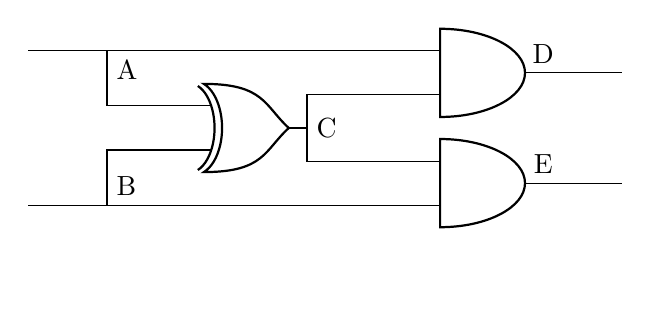
\begin{tikzpicture}
		\node[xor port] (xor)  at (0, 0){};
		\node[and port] (andA) at (3, .7){};
		\node[and port] (andB) at (3,-.7){};
		\draw (andA.in 1)  -- ++(-5, 0)
		      (andB.in 2)  -- ++(-5, 0)
		      (xor.in 1)   -| ++(-1, .7) node [below right] {A}
		      (xor.in 2)   -| ++(-1,-.7) node [above right] {B}
		      (andA.in 2)  -| (xor.out)  node [      right] {C}
		      (andB.in 1)  -| (xor.out)
		      (andA.out) node [above] {D} -- ++( 1, 0)
		      (andB.out) node [above] {E} -- ++( 1, 0)
		      (0,-2); % force a bit of padding
	\end{tikzpicture}
}


\title{Mobile Cryptographic Coprocessor for Privacy-Preserving Two-Party Computation}
\author{Gabriel Kulp}
\date{May 28, 2021}
\institute{kulpga@oregonstate.edu}

\begin{document}

\begin{frame}[plain]
	\centering
	\vspace{1.5cm}

	\large\color{red!70!black}
	Mobile Cryptographic Coprocessor for Privacy-Preserving Two-Party Computation

	\normalsize\vspace{1cm}\color{black}

	Gabriel Kulp

	May 28, 2021

	\vspace{1cm}
	\includegraphics[width=2cm]{logo.png}
\end{frame}
\note{
Hi! My name is Gabriel Kulp and I designed a hardware addon that you can connect to a smartphone to help it do some crazy cryptography faster. Specifically, it evaluates garbled circuits, which are a way to perform computations on different people's private data while keeping it private.

}


\begin{frame}{What is Multi-Party Computation?}
	\begin{itemize}[<+->]
		\item MPC = multi-party computation
		\item Interactive cryptographic protocol
		\item Compute on private inputs
		\item Trust nobody
	\end{itemize}
\end{frame}
\note{
Multi-party computation, or MPC, is a field of cryptography dealing with the design of (advance) of a protocol where some people send cryptographic messages back and forth. (advance) The point of an MPC protocol is to compute the output of some function on private inputs held by each party, but without those parties needing to share their inputs. If you could trust someone to do the computation and keep everyone's inputs secret, then we wouldn't need the cryptography part. (advance) MPC removes the need to trust other parties, but at the cost of lots of math and network traffic.

}


\begin{frame}{Motivation}
	\begin{block}{Who has more money?}
		\begin{itemize}
			\item Millionaires at a party
			\item They don't want to share
			\item No trusted parties
		\end{itemize}
	\end{block}
	\pause
	\begin{block}{Sharing student data}
		\begin{itemize}
			\item Dip in Estonian CS degrees
			\item Tech companies poaching?
			\item Data privacy laws
		\end{itemize}
	\end{block}
\end{frame}
\note{
Let's start with why anybody cares about this.

The classic example is that there are two millionaires at a party that want to find out who has more money, but they don't want to say how much money they have. They could whisper in the butler's ear, but he might give tell someone later or give the wrong answer, so they'd rather not trust anybody.

(advance) A real example from Estonia is that a university wanted to ask some tech companies if there was a correlation that would suggest students were getting hired out of college before finishing their degrees. Estonia has strong privacy laws, though, and sharing that kind of student and employee data would be illegal. They were able to execute a multi-party computation to calculate the correlation of their private datasets and learn something that no party could legally have computed on their own.

There are many other examples like these. In the States we have HIPPAA and FERPA to protect healthcare and student records, but there might be some really good data science we could do if institutions could freely share this information. One solution is to use MPC to perform computations on this data without actually sharing it in the clear.

If you're new to cryptography or haven't heard of Garbled Circuits, this probably sounds like black magic. I'm hoping you can come away from my presentation feeling like it's a little less mysterious.

}


\begin{frame}{Vision}
	\begin{block}{Mobile devices}
		\begin{itemize}
			\item Hardware support for cryptography
			\item Banking and video calls
			\item Save the battery!
		\end{itemize}
	\end{block}
\end{frame}
\note{
My vision is to make computations like these more common. Our devices already have hardware support for some cryptographic operations, and that helps us do things like online banking and secure video calling without hurting battery life so much. I'd like to see smartphones and laptops that can efficiently do MPC with each other or cloud services.

}


\begin{frame}
	\centering
	\Huge

	Algorithm
	
	\color{gray}
	\normalsize
	\vspace{5mm}
	
	Software
	
	\vspace{4mm}

	Hardware
\end{frame}
\note{
I will start my presentation with a lot of background information about the algorithm I devoted Fall term to learning about. Then we'll talk about software considerations and design decisions to implement that algorithm, which was basically my Winter term, and then I'll move into the hardware design, which I worked on this Spring term.

The algorithm I'm going to talk about performs a multi-party computation. Specifically, 

}


\begin{frame}
	\centering
	\Huge{Garbled Circuits}

	\normalsize{Andrew Yao, 1986}
\end{frame}
\note{
I'm going to explain the most common technique for general-purpose multi-party computation, called Garbled Circuits.

This protocol was first described by Andrew Yao in 1986 at that year's IEEE Annual Symposium on Foundations in Computer Science. Since then, the cryptography community has worked out several major improvements to this protocol, including work by my advisor, Dr. Rosulek, in 2015. These improvements would make up another entire presentation, so I'll basically gloss over them for now and describe the core protocol.

}


\begin{frame}[t]{Basic Concepts}
	\begin{columns}
		\begin{column}{.75\textwidth}
			\begin{block}{Boolean Gates}
				\begin{itemize}
					\item Performs operation
					\item AND, XOR, etc.
					\item Considers inputs to choose output
				\end{itemize}
			\end{block}
			\pause
			\begin{block}{Boolean Circuits}
				\begin{itemize}
					\item Connect gates with wires
					\item Output of one is input for another
					\item Performs computation
				\end{itemize}
			\end{block}
		\end{column}
		\begin{column}{.25\textwidth}
			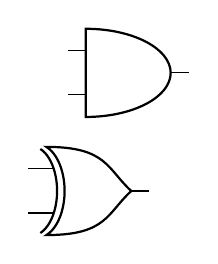
\begin{tikzpicture}
				\pause[0]
				\node[and port] (and) at (.5, 1.5){};
				\node[xor port] (xor) at (0, 0){};
			\end{tikzpicture}
		\end{column}
	\end{columns}
\end{frame}
\note{
To start describing how this works, I'm going to first explain Boolean logic gates of all things. A gate performs a logic operation on its inputs, like AND or exclusive-OR. The gate's job is to observe the values on its input wires and decide what value to put on its output wire.

When you chain these together, you get (adv) a Boolean circuit. Boolean circuits can compute any math expression, but it might take a lot of gates.

}


\begin{frame}{What's Garbling?}
	\centering
	\newcommand*\changingline{}
	\newcommand*\changingbox{draw}
	\only<2->{\renewcommand{\changingline}{[dashed, black!10!white]}}
	\only<2->{\renewcommand{\changingbox}{black!10!white}}
	\begin{tikzpicture}[
		clearbox/.style={rectangle, draw, thick, minimum size=10mm},
		clearIO/.style={rectangle, thick, minimum size=10mm},
		garbledbox/.style={rectangle, draw, thick, minimum size=15mm,align=center},
		garbledIO/.style={rectangle, thick, minimum size=15mm, align=center},
		->,  % makes the edges directed
		>=stealth, % makes the arrow heads bold
		line width=.5mm,
		node distance=2cm,
		]
		\node[clearIO] (i)  {Input};
		\node[clearbox, right=of i,\changingbox] (c) {Circuit};
		\node[clearIO, right=of c] (o) {Output};
		\draw \changingline{} (i) -- (c);
		\draw \changingline{} (c) -- (o);
		\pause
		
		\node[garbledbox, below=of c] (gc) {Garbled \\ Circuit};
		
		\node at ($(c)+(0,-1.33cm)$) [
			top color=black!10!white,
			bottom color=red,
			single arrow,
			minimum height=2cm,
			minimum width=10mm,
			inner sep=0mm,
			single arrow head extend=.1mm,
			rotate=270, single arrow
		] {};

		\pause
		\node[garbledIO, below=of i] (gi) {Garbled \\ Input};
		\draw[red] (i)  -- (gi);
		\pause
		\draw[blue] (gi) -- (gc);
		\pause
		\node[garbledIO, below=of o] (go) {Garbled \\ Output};
		\draw[blue] (gc) -- (go);
		\pause
		\draw[red] (go) -- (o);

	\end{tikzpicture}
\end{frame}
\note{
Evaluating a circuit with the Garbled Circuits protocol requires starting with a normal circuit. Here's what that looks like. An input is converted to something you can put into the circuit on the left side, then the input is propagated through the circuit, and the output comes out the right side.

The garbled circuits protocol is split into two roles. There's the garbler, who I'll call Alice and draw with red, and the evaluator, who I'll call Bob and draw with blue. Alice has to first garble the circuit. (advance) Obviously you don't know what that means yet, but for now it's just a secret transformation. Next, (advance) she works with Bob, who doesn't know the secret transformation, to turn the circuit's input into a garbled input. Alice and Bob both supply part of the circuits input. Bob then puts this input into the garbled circuit (advance), and follows the calculation blindly, since he doesn't know the transformation, to yield the (advance) garbled output. Finally, (advance), Alice helps him turn the garbled output back into the real output, since she's the only one who knows exactly how the circuit was garbled.	

Don't get too scared by this picture just yet. I'm just showing you a roadmap for now and then I'll show the picture again once I've explained what all the pieces mean.

}


\begin{frame}{Boolean Circuit}
	\centering
	\examplecircuit
	\pause
	\begin{columns}
		\begin{column}{.3\textwidth}
			\centering
			\begin{tabular}{c c | c}
				A & B & C \\
				\midrule
				0 & 0 & 0 \\
				0 & 1 & 1 \\
				1 & 0 & 1 \\
				1 & 1 & 0 \\
			\end{tabular}
		\end{column}
		\pause
		\begin{column}{.3\textwidth}
			\centering
			\begin{tabular}{c c | c}
				A & C & D \\
				\midrule
				0 & 0 & 0 \\
				0 & 1 & 0 \\
				1 & 0 & 0 \\
				1 & 1 & 1 \\
			\end{tabular}
		\end{column}
		\pause
		\begin{column}{.3\textwidth}
			\centering
			\begin{tabular}{c c | c}
				B & C & E \\
				\midrule
				0 & 0 & 0 \\
				0 & 1 & 0 \\
				1 & 0 & 0 \\
				1 & 1 & 1 \\
			\end{tabular}
		\end{column}
	\end{columns}
\end{frame}
\note{
Let's start with a closer look at what exactly a circuit is.

Here's an example of a simple boolean circuit. The input wires are on the left side labeled A and B, the output wires are on the right, D and E. All the logic flows from left to right, with no outputs looping back to the left. Gates are referred to by the ID of their output, so the one on the left is called Gate C.

(adv) Gate C is an XOR gate and this table describes how it works. The two input wires on the left of the gate are the A and B columns, and the output is C. Each row of the table shows the output for one combination of inputs.

(advance) And here's a table for Gate D, an AND gate, (adv) and here's the same table for Gate E, which is also an AND gate.

(draw on slides) Let's walk through this just to be very explicit. Let's assign a label of 0 to wire A and a label of 1 to wire B to form our inputs. We can't figure out the outputs D and E yet, since those gates rely on C which we don't have.

We can figure out what label to put on wire C by looking at the table for gate C on the left. From the second row, we can see that the label on wire C should be 1.

Now we know everything required to evaluate the last two gates and find the output of the computation.

(clear drawings) Remember that Bob isn't supposed to know what'g going on, or else he'll be able to figure out Alice's inputs. Now I'm gonna change things up a bit to make that happen. You might be used to thinking of AND and XOR as operations that combine values like True or False and return another value that's either True or False. But actully, there's no need!

}


\begin{frame}{Boolean Circuit (still)}
	\centering
	\examplecircuit
	\begin{columns}
		\begin{column}{.3\textwidth}
			\centering
			\begin{tabular}{c c | c}
				A      & B        & C \\
				\midrule
				$\psi$ & $\phi  $ & $\cap$ \\
				$\psi$ & $\delta$ & $\Leftrightarrow$ \\
				$\pi $ & $\phi  $ & $\Leftrightarrow$ \\
				$\pi $ & $\delta$ & $\cap$ \\
			\end{tabular}
		\end{column}
		\pause
		\newcommand*\rhl{} % row highlight
		\only<4->{\renewcommand{\rhl}{\rowcolor{yellow}}}
		\begin{column}{.3\textwidth}
			\centering
			\begin{tabular}{c c | c}
				A      & C                 & D \\
				\midrule
				$\psi$ & $\cap$            & $\forall$ \\
				$\psi$ & $\Leftrightarrow$ & $\forall$ \\
				$\pi $ & $\cap$            & $\forall$ \\
				\rhl$\pi $ & $\Leftrightarrow$ & $\varnothing$ \\
			\end{tabular}
		\end{column}
		\pause
		\begin{column}{.3\textwidth}
			\centering
			\begin{tabular}{c c | c}
				B        & C                 & E \\
				\midrule
				$\phi  $ & $\cap$            & $\geqq$ \\
				$\phi  $ & $\Leftrightarrow$ & $\geqq$ \\
				$\delta$ & $\cap$            & $\geqq$ \\
				$\delta$ & $\Leftrightarrow$ & $\pitchfork$ \\
			\end{tabular}
		\end{column}
	\end{columns}
	\pause
\end{frame}
\note{
Here I've replaced the 0 and 1 values with arbitrary symbols. Pi and Phi and arrows don't mean anything on their own. They still describe a binary operation, though.

Of course if the C wire is going to be labeled with either a cap or arrows, then gates D and E need to be expecting those kinds of labels as inputs.

(adv) So this table shouldn't be a surprise. The possible labels on the A wire are still Psi and Pi, and we already knew from the previous truth table that the possible labels on the C wire are cap and arrows.

(adv) And this table really shouldn't be a surprise.

(draw) Psi and Delta



This is going to be useful for evaluating a circuit blindly, but there's actually another two steps before we can call this circuit properly garbled.

Remember that Bob isn't supposed to figure out Alice's input.

Right now Bob can figure out from this row (adv) that Pi and arrows must both mean True. You can tell this for two reasons. First, the tables are always in the same order, so the last entry always means both inputs are True. Second, even though the output symbols are arbitrary, you can still tell that there are three upside-down A's and only one slashed circle. Since this is an AND gate, you only get a different output when both inputs are True, so the different output on the bottom row must be when both inputs are True.

Since Bob knows that arrows on wire C mean True, and he knows his input, he can figure out that Delta means false, meaning he figured out Alice's input. Which is a problem.

We can solve the first problem by permuting the rows randomly, but the second problem requires a new trick.

}

\begin{frame}{Symmetric-Key Encryption}
	\begin{columns}
		\begin{column}{.4\textwidth}
			\centering
			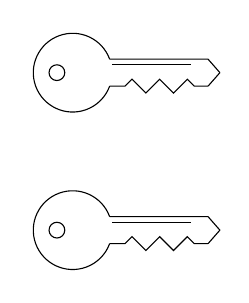
\begin{tikzpicture}
				\bigkey{0,1}
				\bigkey{0,-1}
			\end{tikzpicture}
		\end{column}
		\begin{column}{.6\textwidth}
			\begin{itemize}
				\item Each lock has one key
				\item Each box has two locks
				\item Put anything inside box
			\end{itemize}
		\end{column}
	\end{columns}
\end{frame}
\note{
That trick is symmetric-key encryption, so I need to very briefly cover what it does. Everything will be encrypted with two keys, so you can picture a box that has two locks on it, and you need both keys to open it. You can put whatever you want inside the box of course, and that's where things get really cool.

}

\newcommand{\enc}[3]{\(\textrm{enc}(\{#1, #2\}, #3)\)}
\begin{frame}{Garbling a Gate}
	\centering
	\begin{tabular}{c c | r@{} l@{} l@{} l} % I know this is gross. If it works it works!
		A      & C                 & & D & \\
		\midrule
		$\psi$ & $\cap           $ & $\textrm{enc}(\{$ & $\psi,            \hspace{.7mm}\cap$ & $\},\forall    $ & ) \\
		$\psi$ & $\Leftrightarrow$ & $\textrm{enc}(\{$ & $\psi,            \Leftrightarrow  $ & $\},\forall    $ & ) \\
		$\pi $ & $\cap           $ & $\textrm{enc}(\{$ & $\hspace{.5mm}\pi,\hspace{.7mm}\cap$ & $\},\forall    $ & ) \\
		$\pi $ & $\Leftrightarrow$ & $\textrm{enc}(\{$ & $\hspace{.5mm}\pi,\Leftrightarrow  $ & $\},\varnothing$ & )
	\end{tabular}
	\color{white} % just for spacing to align with the next one
	\[\textrm{dec}(\{\pi, \cup\}, 1101110001) = \forall\]
	$\pi = 0000101110, \cap = 1100100010$
\end{frame}
\note{
Alright, so here's the breakthrough. What if we encrypt the output of each row? And we'll use the input wire labels on their own to form the key! Bob, who's evaluating the circuit, will only know the current label on wire A, called the "active" label; he doesn't know what the other label could be since it's arbitrary. Same with wire C.

}

\begin{frame}{Garbling a Gate}
	\centering
	\begin{tabular}{c c | c}
		A                   & C                              & D \\
		\midrule
		\color{gray} $\psi$ & \color{gray} $\cap$            & $0111010110$ \\
		\color{gray} $\psi$ & \color{gray} $\Leftrightarrow$ & $0010111011$ \\
		\color{gray} $\pi $ & \color{gray} $\cap$            & $1101110001$ \\
		\color{gray} $\pi $ & \color{gray} $\Leftrightarrow$ & $0010001100$
	\end{tabular}
	\color{white} % just for spacing to align with the next one
	\[\textrm{dec}(\{\pi, \cup\}, 1101110001) = \forall\]
	$\pi = 0000101110, \cap = 1100100010$
\end{frame}
\note{
Also, Bob can't actually see all the symbols on the input side of the table, and he can't see inside the encrypted values, either; they look random until decrypted.

There's still the problem where Bob can figure out too much from the order of the table. To solve this, we do one last operation and permute the table randomly.

}

\begin{frame}{Garbling a Gate}
	\newcommand*\rhl{} % row highlight
	\only<2->{\renewcommand{\rhl}{\rowcolor{yellow}}}
	\centering
	\begin{tabular}{c c | c}
		A                   & C                              & D \\
		\midrule
		\rhl\color{gray}$\pi$&\color{gray} $\cap$            & $1101110001$ \\
		\color{gray} $\psi$ & \color{gray} $\cap$            & $0111010110$ \\
		\color{gray} $\psi$ & \color{gray} $\Leftrightarrow$ & $0010111011$ \\
		\color{gray} $\pi $ & \color{gray} $\Leftrightarrow$ & $0010001100$
	\end{tabular}
	\pause
	\[\textrm{dec}(\{\pi, \cap\}, 1101110001) = \forall\]
	\pause
	$\pi = 0000101110, \cap = 1100100010$
\end{frame}
\note{
So if Bob has Pi on wire A and Cap on wire C, then the only entry he has a valid key for is this one (adv), which decrypts to the upside-down A. He doesn't know that the other options are Psi and arrows, and he doesn't know that the other output is the slashed circle.

This means that Bob can take the inputs to the gate and figure out the output, but he doesn't learn anything about the semantic value of the arbitrary input or output labels. To be clear, Alice sets all this up and chooses the arbitrary labels and does the encryptions, so she knows exactly what's hiding in here.

If Alice had the inputs to evaluate the circuit, she would know Bob's inputs, which isn't allowed and defeats the whole purpose. So Bob needs to be the one to evaluate the circuit, since he can do it blindly. This of course requires Alice to set things up in such a way that Bob is actually blind. She does this by choosing arbitrary wire labels, encrypting the truth table outputs with the inputs as keys, and then randomly transposing the table.

(adv) Just as a little aside here: the arbitrary labels are larger than one bit, which is how you can make a key from them that's safe against guessing. If they were just private aliases for True and False, it would be trivial to guess-and-check to recover all the output values, so they actually need to be long random numbers.

}


\begin{frame}{What's Garbling?}
	\centering
	\newcommand*\changingline{}
	\newcommand*\changingbox{draw}
	\only<2->{\renewcommand{\changingline}{[dashed, black!10!white]}}
	\only<2->{\renewcommand{\changingbox}{black!10!white}}
	\begin{tikzpicture}[
		clearbox/.style={rectangle, draw, thick, minimum size=10mm},
		clearIO/.style={rectangle, thick, minimum size=10mm},
		garbledbox/.style={rectangle, draw, thick, minimum size=15mm,align=center},
		garbledIO/.style={rectangle, thick, minimum size=15mm, align=center},
		->,  % makes the edges directed
		>=stealth, % makes the arrow heads bold
		line width=.5mm,
		node distance=2cm,
		]
		\node[clearIO] (i)  {Input};
		\node[clearbox, right=of i,\changingbox] (c) {Circuit};
		\node[clearIO, right=of c] (o) {Output};
		\draw \changingline{} (i) -- (c);
		\draw \changingline{} (c) -- (o);
		\pause
		
		\node[garbledbox, below=of c] (gc) {Garbled \\ Circuit};
		
		\node at ($(c)+(0,-1.33cm)$) [
			top color=black!5!white,
			bottom color=red,
			single arrow,
			minimum height=2cm,
			minimum width=10mm,
			inner sep=0mm,
			single arrow head extend=.1mm,
			rotate=270, single arrow
		] {};

		\pause
		\node[garbledIO, below=of i] (gi) {Garbled \\ Input};
		\node[garbledIO, below=of o] (go) {Garbled \\ Output};
		\draw[red] (i)  -- (gi);
		\draw[red] (go) -- (o);

		\pause
		\draw[blue] (gi) -- (gc);
		\draw[blue] (gc) -- (go);

	\end{tikzpicture}
\end{frame}
\note{
Alright, now we can come back to this picture to see what's left. The whole goal here is to evaluate a function. In our case, we represent that function as a boolean circuit.

There are two roles: Alice is the garbler. (adv) She picks a secret translation that she can apply to the circuit, its inputs, and its outputs.

(adv) Bob doesn't know the translation, so he's free to do the computation without leaking any private information.

Perhaps you've noticed a problem, though. How can Bob get the circuit's input to start with? Let's say that Alice's input goes on Wire A and Bob's input goes on Wire B.

}

\begin{frame}{Inputs?}
	\begin{columns}
		\begin{column}{.5\textwidth}
			\centering
			\begin{tabular}{c c | c}
				A      & B        & C \\
				\midrule
				$\psi$ & $\phi  $ & $\cap$ \\
				$\psi$ & $\delta$ & $\Leftrightarrow$ \\
				$\pi $ & $\phi  $ & $\Leftrightarrow$ \\
				$\pi $ & $\delta$ & $\cap$ \\
			\end{tabular}
		\end{column}
		\begin{column}{.5\textwidth}
			\centering
			\begin{tabular}{c c c}
				Wire & True   & False \\
				\midrule
				A    & $\psi$ & $\pi$ \\
				B    & $\phi$ & $\delta$
			\end{tabular}
		\end{column}
	\end{columns}
\end{frame}
\note{
Here's a table from earlier on the left and Alice's arbitrary label choices on the right.

Alice chooses these arbitrary labels to correspond to True and False, and she makes these choices for every wire.

Bob's the one to actually evaluate the circuit, so he needs to know which inputs to use.

Alice can just give Bob the right key for her own input A, since Bob doesn't know what it means. Only Alice can see the table on the right, so if she knows that her input is False, she just gives Bob Pi and he doesn't know what it means. He can still plug it into the table blindly, though.

Alice can't give Bob both options for wire B, because then he would learn too much about the gates. He could try evaluating the circuit with both inputs and figure out more that what they agreed on. At the same time, Bob can't just ask Alice for whatever label corresponds to True, since then Alice would know Bob's input and the whole thing would be pointless.

}


\usetikzlibrary{arrows}
\begin{frame}{The Oblivious Transfer}
	\centering
	\newcommand*\secretA{``hello''}
	\newcommand*\secretB{``world''}
	\only<5->{\renewcommand{\secretA}{$\phi$}}
	\only<5->{\renewcommand{\secretB}{$\delta$}}
	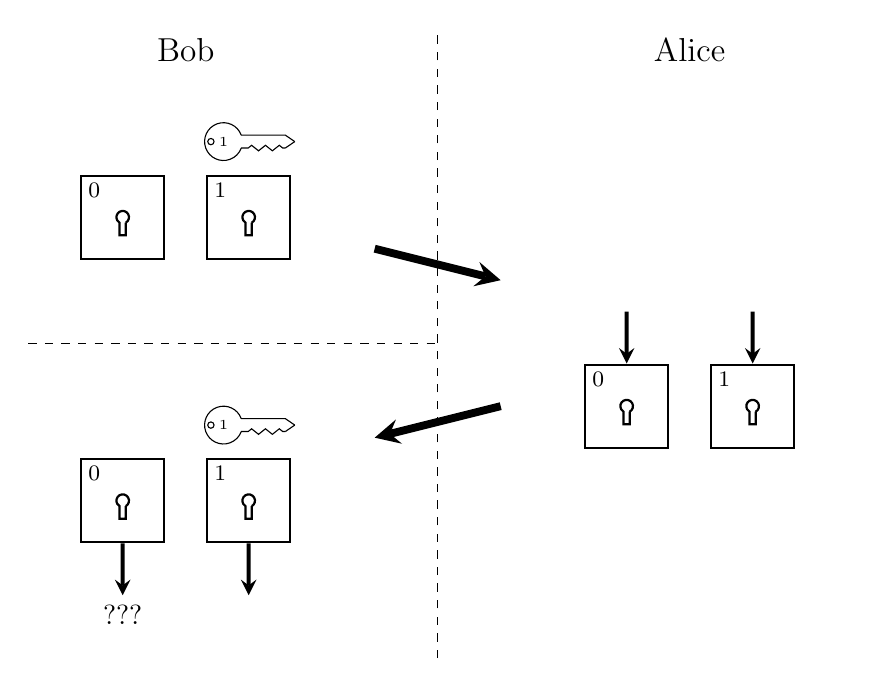
\begin{tikzpicture}[ scale=.8,
			IOarrow/.style={->, >=stealth, line width=.5mm},
			flowarrow/.style={->, >=stealth, line width=1mm, auto}
		]
		\draw[dashed] (0,-5) -- (0,5);

		\draw (-4,5) node [below] {\large{Bob}};
		\draw (4,5)  node [below] {\large{Alice}};
		\pause
		
		\lockshape{-5,2}{0} % step 1
		\lockshape{-3,2}{1}
		\pause
		% 1 -> 2 arrow
		\draw[flowarrow, bend right=20] (-1,1.5) -- (1,1);

		\lockshape{5,-1}{1} % step 2
		\draw (5,.5) node [above] (txt) {\secretB};
		\draw[IOarrow] (txt) -- (lastBox);
		\lockshape{3,-1}{0}
		\draw (3,.5) node [above] (txt) {\secretA};
		\draw[IOarrow] (txt) -- (lastBox);
		\pause
		% key from step 1
		\littlekey{-3,3.2}{1}

		% horizontal divider
		\draw[dashed] (-6.5,0) -- (0,0) (6.5,0);
		% 2 -> 3 arrow
		\draw[flowarrow, bend right=20] (1,-1) -- (-1,-1.5);

		\lockshape{-5,-2.5}{0} % step 3
		\draw (-5,-4) node [below] (txt) {???};
		\draw[IOarrow] (lastBox) -- (txt);
		\lockshape{-3,-2.5}{1}
		\draw (-3,-4) node [below] (txt) {\secretA};
		\draw[IOarrow] (lastBox) -- (txt);
		\littlekey{-3,-1.3}{1}

	\end{tikzpicture}
\end{frame}
\note{
The solution is a really fun cryptographic primitive called an Oblivious Transfer, or OT. If Alice and Bob perform an OT, then Bob can ask for just one label, and Alice sends it to him. The cool part is that Alice doesn't know which one he asked for, and Bob doesn't know anything about the label he didn't receive!

(adv) You can picture this as Bob sending Alice two empty boxes, labeled 0 and 1. (adv) Alice puts messages in each box, locks them, and sends them back. (advance) But Bob only made the key to box 1, a choice he made before sending anything to Alice. Alice doesn't know which message Bob got, since the locks on the boxes look the same to her. Bob doesn't learn anything about the other message since this whole thing is set up so that he can only ever open one box.

Now imagine that the messages that Alice puts in the boxes are actually the arbitrary True and False labels for the circuit input. (adv) This is how Bob can ask for the labels he needs without Alice learning his input.

}

\begin{frame}{Putting it All Together}
	\pause
	\begin{itemize}[<+->]
		\item Alice generates labels and tables
		\item Alice sends her inputs to Bob
		\item Bob gets his inputs with OT
		\item Bob evaluates the circuit
	\end{itemize}
\end{frame}
\note{
So let's put all those pieces together. First, (advance) Alice garbles every gate by generating a bunch of wire labels and encrypting gate outputs, where each output is the input to another gate. Next, (advance) Alice sends the labels that correspond to her inputs over to Bob, since he doesn't know which labels mean True and which mean False. Then, (advance) Bob uses an oblivious transfer to get the True and False labels for his input from Alice. Since it's oblivious, Alice doesn't know which labels he got, so neither of them know the other's inputs.

Finally, (advance) Bob evaluates the circuit blindly by decrypting entries to any truth tables that he has both inputs for until he's evaluated every gate. At the end, he can just ask Alice what the outputs mean and she'll tell him whether each label means True or False. There are ways to make sure she doesn't lie, but we'll assume they're on good terms and just want some privacy.

}


\begin{frame}
	\centering
	\color{gray}
	
	Algorithm
	
	\Huge\color{black}
	\vspace{2mm}

	Software

	\normalsize\color{gray}
	\vspace{5mm}

	Hardware
\end{frame}
\note{
Alright, that's the first section done! It's the longest one, so don't worry.

Next I'll talk about how I implemented Garbled Circuits in software and why I made the design decisions that I did.

After that, I'll talk about the actual coprocessor that I designed and how I tested it.

}

\begin{frame}{System Setup}
	\centering
	
	\newcommand*\alice{Alice}
	\only<2->{\renewcommand{\alice}{Garbler}}
	\only<3->{\renewcommand{\alice}{Cloud}}
	\newcommand*\bob{Bob}
	\only<2->{\renewcommand{\bob}{Evaluator}}
	\only<3->{\renewcommand{\bob}{Smartphone}}
	\newcommand*\net{Connection}
	\only<3->{\renewcommand{\net}{Internet}}
	
	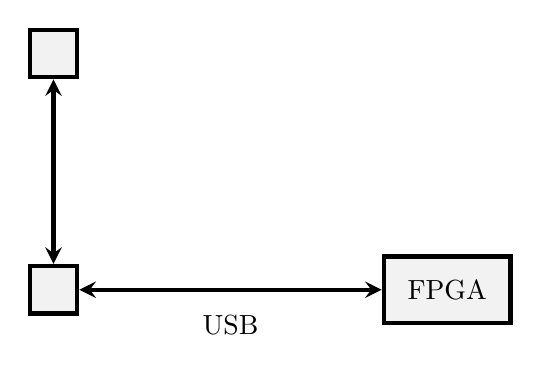
\begin{tikzpicture} [
			%scale=1.3, every node/.style={transform shape},
			box/.style={rectangle, draw, ultra thick, fill=black!5!white},
			arrow/.style={ultra thick, <->, >=stealth},
			inner sep=3mm, align=center
		]
		\node at (0,3) [box] (cloud) {\alice};
		\node at (0,0) [box] (phone) {\bob};
		\draw [arrow] (cloud) -- (phone) node[midway, right] {\net};
		\pause
		\pause
		\pause
		\node at (5,0) [box] (fpga) {FPGA};
		\draw [arrow] (phone) -- (fpga)  node[midway, below] {USB};
	\end{tikzpicture}

\end{frame}
\note{
So here's what I've talked about so far. Alice and Bob are separate parties, but they do this computation together. They need some connection to do the oblivious transfer and for Alice to send the garbled truth tables to Bob.

(adv) In more general terminology, let's remember that Alice is the garbler and Bob is the evaluator.

(adv) As I mentioned at the beginning, my goal is to allow mobile devices to perform MPC calculations more efficiently, and the use case that I focused on is the cloud-computing model. Since Alice has a lot more computation to do than Bob, she's going to have a big datacenter in the cloud. There's already academic work focused on that side of the equation, so I'm going to instead help Bob do his part more efficiently.

(adv) And I'm accomplishing that by giving Bob an extra device to help him out.

I need to program all three of these boxes, but in this section we're just talking about the two on the left.

So my software therefore has two parts: one part for the garbler in the cloud (which happens to be my nickname), and the other part for the evaluator, who just has a smartphone. I wrote a unified library for working with MPC problems, and then one script for each role.

The software part was a lot of work, but presenting code is tough for everyone involved, so I'll keep it pretty high-level. Feel free to ask questions at the end if you'd like more details on any of the components I'm about to cover.

}

\begin{frame}{Software Components}
	\begin{itemize}[<+->]
		\item Boolean circuits
		\item Symmetric encryption (AES)
		\item Asymmetric encryption (RSA)
		\item Oblivious transfer
		\item Networking
		\item FPGA connection
	\end{itemize}
\end{frame}
\note{
Since I approached this by writing a library first, I had to figure out what components the library would have.

First, I needed a representation of a normal, non-garbled, Boolean circuit. That includes the ability to evaluate it for testing and to read a circuit definition from a file. I'll show you what that looks like in a moment. Computers are generally good at this sort of thing, so it was probably a day or two of work to get to the point where I could download a circuit definition, choose some inputs, and calculate the output. This step is important so that I have a baseline to compare to when I start garbling.

(adv) Next, I needed a way to encrypt and decrypt rows of truth tables. I could have used a standard system library like OpenSSL to do this, but I decided to implement it myself as a learning exercise since I'd have to program it from scratch in hardware later anyway.

(adv)(adv) Of course evaluating the circuit is only part of the process. Bob still needs to securely get all the circuit inputs, and that requires oblivious transfers, which require asymmetric encryption, also called public key cryptography. So that's another library I have to write. I first wrote the public key crypto part, and then I built the oblivious transfer protocol from it. I chose to implement this part only in software, but I still wanted to write it all myself as part of my learning process.

(adv) All of this needs to happen at a distance, so I need a way to open a connection between two computers, serialize everything, send it through, deserialize on the other end, and then use the received values. It turns out that most of the hard part here is already handled by the operating system with sockets. You just call a system function or two to open a socket between the devices, then anything you put in one side comes out the other side. I still had to decide how to serialize things and what order things get sent and all that, though.

(adv) Finally, I need to write this software with the presence of an FPGA in mind. This means that I need to design Bob's logic in such a way that moving the computation to the coprocessor doesn't disrupt the rest of the program's structure. This ended up being easier than it sounds and basically boils down to streaming everything.

My first iteration first reads the entire circuit, then Alice garbled it and sent it to Bob, and once he received it, Bob evaluated the circuit. This approach doesn't work well for the FPGA since it would need to store the whole circuit onboard, and it doesn't have much memory. Instead, I streamed everything, so the first gate is read from the definition file, garbled, and sent before the next line is read. Then Bob just has to keep up with this constant stream. For comparison, doing a single integer division of 64-bit numbers takes 30,000 gates, and doing a floating point square root takes over 200,000 gates.

}


\begin{frame}{Circuit Definition}
	\centering
	\includegraphics[height=.8\textheight]{../figures/screenshot-circuit.png}
\end{frame}
\note{
As promised, here's what a circuit defition file looks like. The whole file is 16,956 lines long, so I've just included the first 16 lines. The grey numbers on the left are just line numbers, so they aren't part of it.

The first line tells you the total number of gates and wires. The next line says there are 2 inputs, and each is 64 wires wide. Line 3 says there's one output that's 64 wires wide.

Then comes the long part with the actual circuit. Each line is one gate and the text on the right side says what kind of gate it is.

Line 5 says that there are 2 inputs and 1 output. The inputs are wires 127 and 126, and the output is wire 128. I used letters to refer to wires since that's easier for humans, but here we're using numbers for scalability.

None of these gates have outputs less than 128 since the first 128 wires, numbered from zero to 127, are the two 64-bit inputs.

}


\begin{frame}{Python}
	\centering
	\includegraphics[width=\textwidth]{../figures/screenshot-python.png}
\end{frame}
\note{
And here's a snippet from the software implementation of Bob's role as the evaluator. I wrote the software in Python mostly because I'm comfortable with that language and how to debug it.

On the very first line you can see the thing I was just talking about. "circuit.gates" is a generator, meaning it produces a list on the fly. This block of code then deals with those gates on the fly in a streaming approach.

You can see that there are three blocks here, one for each type of gate. Unfortunately I don't have enough time to go into the optimization techniques that researchers have figured out over time, so the rest of the code probably doesn't make much sense. I'm happy to talk about this stuff in more detail at the end, or at the Engineering Expo on the 4th if you come by my room.

}


\begin{frame}
	\centering
	\color{gray}
	
	Algorithm
	
	\vspace{5mm}
	
	Software
	
	\Huge\color{black}
	\vspace{2mm}

	Hardware
\end{frame}
\note{
And that's it for the software section!

See? We're moving right along.

Now we can talk about the hardware!

}


\begin{frame}{What's an FPGA?}
	\centering
	\begin{tikzpicture}[scale=.97, every node/.style={transform shape}] % 7pt too wide at full size...
		\node (image) {\includegraphics[width=.5\textwidth]{../figures/fabric-full.png}};
		\node at (5.75,1)  [rectangle, align=center] {Field-Programmable\\Gate Array};
		\node at (5.75,-1) [rectangle, align=center] {$\leftarrow$ Logic fabric};
		\pause
		\draw[white, fill] (1,0) circle(3.5mm);
		\draw[white, line width=2mm]
			(130:3.1) ++(5,0) coordinate(top)
			(-130:3.1)++(5,0) coordinate(bottom)
			(130:.25)  ++(1,0) -- (top)
			(-130:.25) ++(1,0) -- (bottom);
		\begin{scope}[even odd rule]
			\draw[white, fill] (5,0) circle(3.2cm);
			\draw[black, ultra thick, fill=white] (5,0) circle(3.1cm);
			\clip (5,0) circle(3cm);
			\node (image) at (5,0) {\includegraphics[height=6cm]{../figures/fabric-zoom.png}};
		\end{scope}
		\draw[black, ultra thick]
			(130:3.1) ++(5,0) coordinate(top)
			(-130:3.1)++(5,0) coordinate(bottom)
			(130:.25)  ++(1,0) -- (top)
			(-130:.25) ++(1,0) -- (bottom);
		\draw[black, ultra thick, fill=white] (1,0) circle(2.5mm);
	\end{tikzpicture}
\end{frame}
\note{
FPGA stands for "Field-Programmable Gate Array" it's a kind of chip that implements reconfigurable logic. My coprocessor design runs on an FPGA rather than going through the prohibitively expensive process of manufacturing a ``real'' single-purpose chip. The ``gate array'' part of the name means that the chip is made of a grid of general-purpose elements. This part of the chip is called the fabric.

The ``field-programmable'' part of the name means that these connections can be reconfigured on-the-fly after the chip has been manufactured and shipped. I used this reprogramming capability to test each iteration of my design.

Zooming in (adv), you can see diagonal wires representing a connection between the bus lines and components internal to each element. There are several types of elements distributed across the fabric, including elements specifically for robust input and output, clock signal generation, digital signal processing, and several types of memory. Most tiles on the fabric are "basic elements", which contain registers and configurable lookup tables. This means that all 5280 basic elements can be configured to behave as a logic gate, a memory cell, an interconnect, or often all three.

}

\begin{frame}{Workflow}
	\centering
	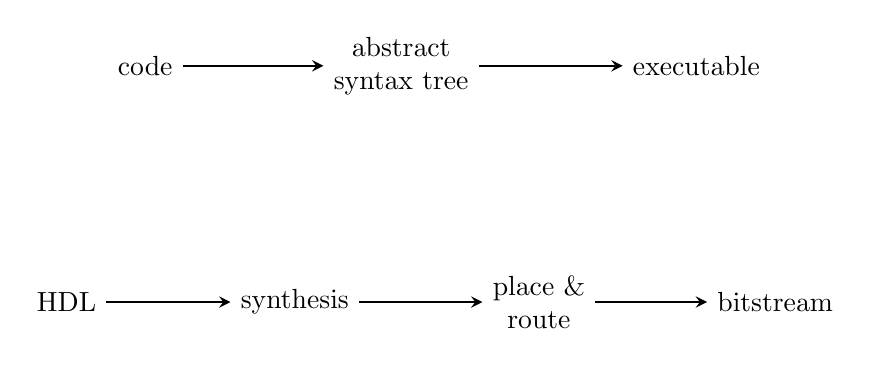
\begin{tikzpicture}[
			every node/.style={align=center,rectangle},
			every path/.style={->,>=stealth,thick}
		]
		\node at (1,0) (code) {code};
		\node at (4.25,0) (ast) {abstract\\syntax tree};
		\node at (8,0) (exe) {executable};
		\draw (code) -- (ast);
		\draw (ast) -- (exe);

		\pause

		\node at (0,-3) (hdl) {HDL};
		\node at (2.9,-3) (syn) {synthesis};
		\node at (6,-3) (pnr) {place \&\\route};
		\node at (9,-3) (bin) {bitstream};
		\draw (hdl) -- (syn);
		\draw (syn) -- (pnr);
		\draw (pnr) -- (bin);
	\end{tikzpicture}
\end{frame}
\note{
Some of you will be very familiar with the way that code turns into an executable. The compiler reads the source code and builds an abstract syntax tree that encodes the control flow and data types and everything. Then it does the process again backwards, turning the abstract representation into a concrete one, specifically CPU instructions. Then to execute the program, these instructions are loaded into memory and the computer performs each action in the list.

Designing hardware is similar in some ways. (adv) Instead of starting with source code, you start with a hardware description language, or HDL, like Verilog, which is used to define state machines and combinational logic at the register-transfer level of abstraction.

Synthesis is the process of turning this description into an abstract hardware definition that's a lot like the abstract syntax tree from software compilers.

Place \& route is the process of placing circuit components onto elements of the FPGA fabric and routing connections between these components like we saw in the picture on the previous slide.

Once the final FPGA configuration has been determined, it's serialized into a format that the FPGA chip can read to configure itself. This is unimaginatively called the bitstream.

}


\begin{frame}{Verilog}
	\centering
	\includegraphics[height=.8\textheight]{../figures/screenshot-verilog.png}
\end{frame}
\note{
Here's a snippet of Verilog code. You can see at the top that this is an "always" block, and everything inside happens on the positive edge of the clock signal, meaning when that wire's voltage goes from low to high. Everything inside the "always" block happens at the same time, so this isn't a list of sequential instructions.

The first part inside is a block to handle resetting, and then after that, there's a case statement that forms a state machine.

This particular snippet is from the memory controller that fetches wire labels for each gate's inputs. I just included it to put a picture in your head of what it looks like to describe hardware.

}


% spellchecker: ignore CISC
\begin{frame}{Design decisions}
	\begin{itemize}[<+->]
		\item CISC (complex instruction set computer)
		\begin{itemize}
			\item Only six instructions
			\item I/O: set address, read, write
			\item Gates: AND, XOR, BUF
		\end{itemize}
		\item No program counter
		\item No branches
		\item Memory-memory architecture
		\item Event-based
		\item Extensible
	\end{itemize}
\end{frame}
\note{
Okay, let's talk about what I actually did and try to describe it in normal CPU terms. To begin with, I would classify it as a CISC design, which means that each instruction does a lot of work. This is compared to a RISC, or reduced instruction set, computer, which has instructions that each only do a little thing. (adv) there are only 6 instructions. Three are for handling input and output, and three compute on data inside already. (adv) you can picture the processor's memory like a tape. Once the smartphone has the circuit inputs, it sets the tape's read/write head at the beginning and sends some data for it to write at that location. At the end, the head gets moved to the output of the garbled circuit and the chip reads the data out to the smartphone.

(adv) The three instructions for computing on data already inside are for three kinds of logic gates. I've already talked about AND and XOR gates, but I also support the buffer gate, which just copies its input to its output. You'll have to trust me that that's useful here. In the case of the AND gate, that single instruction means that the coprocessor needs to do two memory lookups, an AES encryption, an XOR, and then write the result back to a new location in memory. It's a similar story for the other gates.

(adv) Unlike a full-fledged CPU, there's no program counter. Usually CPUs read their own instructions, so they need a register to store the location of the next instruction to read. In my case though, instructions are streamed in over USB.

(adv) This also means that there are no branching instructions. In other words, the coprocessor never needs to make a decision. Normally a CPU would be able to change its program counter dynamically based on conditions, but none of that happens here.

(adv) I kind of already said this, but I would classify this is a memory-memory architecture, meaning that its instructions describe an operation to do to values stored in memory. This is in contrast to a register-memory architecture which executes operations where one operand is in a register and the other can be in memory. There are also load-store architectures which only do operations between registers and require separate instructions to move data from memory to registers or back again.

(adv) I kind of made this term up, but I'd also call my design event-based, meaning that there's no central control unit orchestrating how the various parts work together. Instead those parts talk directly to each other. For example, the memory controller waits to store a value until the encryption unit raises an event saying it's done computing. I'm borrowing the term from event-based programming, where you write modules that subscribe to events that other modules can raise. There might be a better name for this in hardware, but I don't know it.

I individually pipelined each of these modules that can be, but I can't pipeline between them because everything here is a pipeline hazard, meaning the input to each module depends on the output of the last. Also since every value from memory appears random, speculative execution isn't much of an option.

(adv) Finally, I'll assert that this event-based idea actually does a lot to make the design extensible. Right now I'm just using on-board memory, but if I wanted to use a memory expansion, I would need to replace the memory controller module. Since the next step waits until memory finishes, that means that I don't need to change anything else about the design if the new memory controller is faster or slower than the old one. If there was a central control unit, I might need to adjust counters to account for the new timing to get everything synchronized.

Alright, that's all I have to say on that topic for now. Again, feel free to ask me anything about this stuff at the end. We're almost there!

}


\begin{frame}{Results}
	\begin{itemize}[<+->]
		\item I understand Garbled Circuits!
		\item Proof: software works
		\item Proof: hardware works
		\item $62\times$ speedup compared to software \only<5->{(maybe?)}
		\item<6-> Same battery life
	\end{itemize}
\end{frame}
\note{
Honestly my primary goal in this project was to understand Garbled Circuits. I can confidently say that I do!

(adv) For proof I offer my functional software implementation

(adv) For further proof I offer my functional hardware implementation.

(adv) In fact, it seems like my implementations are even better than just functional! Depending on how you measure it, the smartphone is 26 times faster when it uses the coprocessor than when it does everything in software on its own. (adv) Now that might just be because my software implementation is terrible. In fact I know that there's a terrible bottleneck in the serial library that I use to communicate with the FPGA, which I'm fine with because I didn't write it! Right now the coprocessor actually sits idle for around 5000 clock cycles waiting for the phone to send the next instruction. I know from testing that the serial connection is fast enough to send instructions back-to-back, but I ran out of time to do a proper investigation into this. Since instructions take 80 clock cycles to execute on average, that comes out to a 26 times speedup if the smartphone didn't insert those huge gaps.

(adv) As another bonus, the phone's battery life was the same with and without the coprocessor! The particular chip I used is actually marketed for low-power uses, so it's not super surprising, but I was still happy to see that.

}


\begin{frame}
	\Huge\centering
	Questions?

	\vspace{2cm}
	\includegraphics[width=2cm]{logo.png}
\end{frame}
\note{
And that's it! Now you can see my logo again and hopefully it makes a little more sense. It's a logic gate inside a chip that represents the FPGA. Anyway, I'll take questions now!

}

\end{document}
